%%%%%%%%% INTRODUCTION
\section{Introduction}
\label{sec:intro}

Facial keypoint detection, the task of localizing and identifying key facial landmarks in images, serves as a fundamental component in various computer vision applications such as facial recognition, emotion analysis, and facial expression synthesis. Further, the accurate localization of key facial landmarks such as eyes, nose, and mouth corners is crucial for tasks like face alignment and tracking, enabling advancements in human-computer interaction, biometrics, and augmented reality.  Despite significant advancements in recent years, accurate and robust facial keypoint detection remains a challenging problem due to variations in facial expressions, poses, lighting conditions, and occlusions.~\cite{WANG201850} \\

Traditional approaches to facial keypoints detection often rely on handcrafted features and shallow learning models, which may struggle to capture the complex and subtle patterns present in facial images or generalize well to diverse and complex datasets. With the emergence of deep learning, convolutional neural networks (CNNs) have demonstrated remarkable success in automatically learning hierarchical representations directly from raw pixel data.~\cite{9065279}  However, the success of CNN-based methods heavily depends on the quality and diversity of the training data, as well as the effectiveness of the training process itself.\\

In this paper, we propose a novel approach to enhancing facial keypoints detection performance by integrating several key strategies: image correction and label fine-tuning, stacked generalization of weak learners leveraging a K-fold strategy, and a split pipeline for data processing and training through detection of individual contributing organizers, allowing for exploitation of variance in labeling patterns. To further enhance the robustness of our system, we incorporate image augmentation techniques, artificially expanding the training dataset, thereby improving diversity and generalized performance of each weak learner.\\

To evaluate the effectiveness of our approach, we conduct extensive experiments on a benchmark facial keypoints detection dataset from the 2017 Kaggle competition: \href{https://www.kaggle.com/competitions/facial-keypoints-detection/overview}{Facial Keypoints Detection}.  Competition submissions are scored on the root mean squared error as the standard metric for comparing solution quality:
\begin{equation}
	\text{RMSE} = \sqrt{\frac{1}{N} \sum_{i=1}^N \left(y_i - \hat{y}_i\right)^2}
\end{equation}
Our results demonstrate that the proposed method achieves state-of-the-art performance. Overall, this paper presents a comprehensive framework for improving facial keypoints detection, offering valuable insights into the synergy between data augmentation, ensemble learning, and data processing techniques in the context of computer vision tasks.

%-------------------------------------------------------------------------
\subsection{Related Work}

Facial keypoint detection has been a subject of active research in computer vision for several decades, with a variety of approaches proposed.  Traditional methods often relied on handcrafted features and shallow learning models, such as support vector machines (SVMs) coupled with techniques like Haar cascades or local binary patterns (LBP) for feature extraction~\cite{VIOLAANDJONES2014, 1717463}. \\

In recent years, the rise of deep learning has transformed facial keypoints detection work by enabling end-to-end learning directly from raw (lcalized) pixel data.  CNNs have emerged as the dominant architecture for this task due to their ability to automatically learn hierarchical representations, capturing both low-level features like edges and high-level semantic information~\cite{LECUN2015NATURE}.  Early CNN-based approaches demonstrated promising results on facial keypoints detection tasks, insporing subsequent research in the domain.~\cite{10.1007/978-3-319-10599-4_7} \\

Several studies have focused on enhancing the robustness and accuracy of facial keypoints detection by exploring various aspects of deep learning architectures and training methodologies.  Zhang et al.~\cite{Zhang_2015} introduced a multi-task learning framework that jointly predicts facial keypoints and facial attributes, leveraging shared representations to improve performance. Similarly, Sun et al.~\cite{6619290} proposed a cascaded CNN architecture that refines keypoints predictions iteratively, enabling better handling of occlusions and variations in facial expressions.\\

Ensemble learning techniques have also been applied to facial keypoints detection, aiming to leverage the diversity of multiple models to improve overall performance. Zhang et al.~\cite{wu2017robust} proposed a boosting-based approach that combines weak learners trained on different subsets of the data, effectively reducing generalization errors and enhancing robustness to outliers.  Similarly, Liu et al.~\cite{liu2015deep} explored the use of stacked generalization, combining predictions from multiple base models with a meta-learner to achieve superior performance.\\

While these prior works have made significant contributions to the field, they often focus on individual aspects of the facial keypoints detection pipeline, such as model architecture or training strategy, without fully exploiting the potential synergy between different techniques.  In contrast, our proposed method integrates image augmentation, stacked generalization, and targeted data preprocessing to achieve state-of-the-art performance, highlighting the importance of a holistic approach to addressing the challenges of facial keypoints detection.\\

\begin{figure}[t]
	\centering
	%\fbox{\rule{0pt}{2in} \rule{0.9\linewidth}{0pt}}
	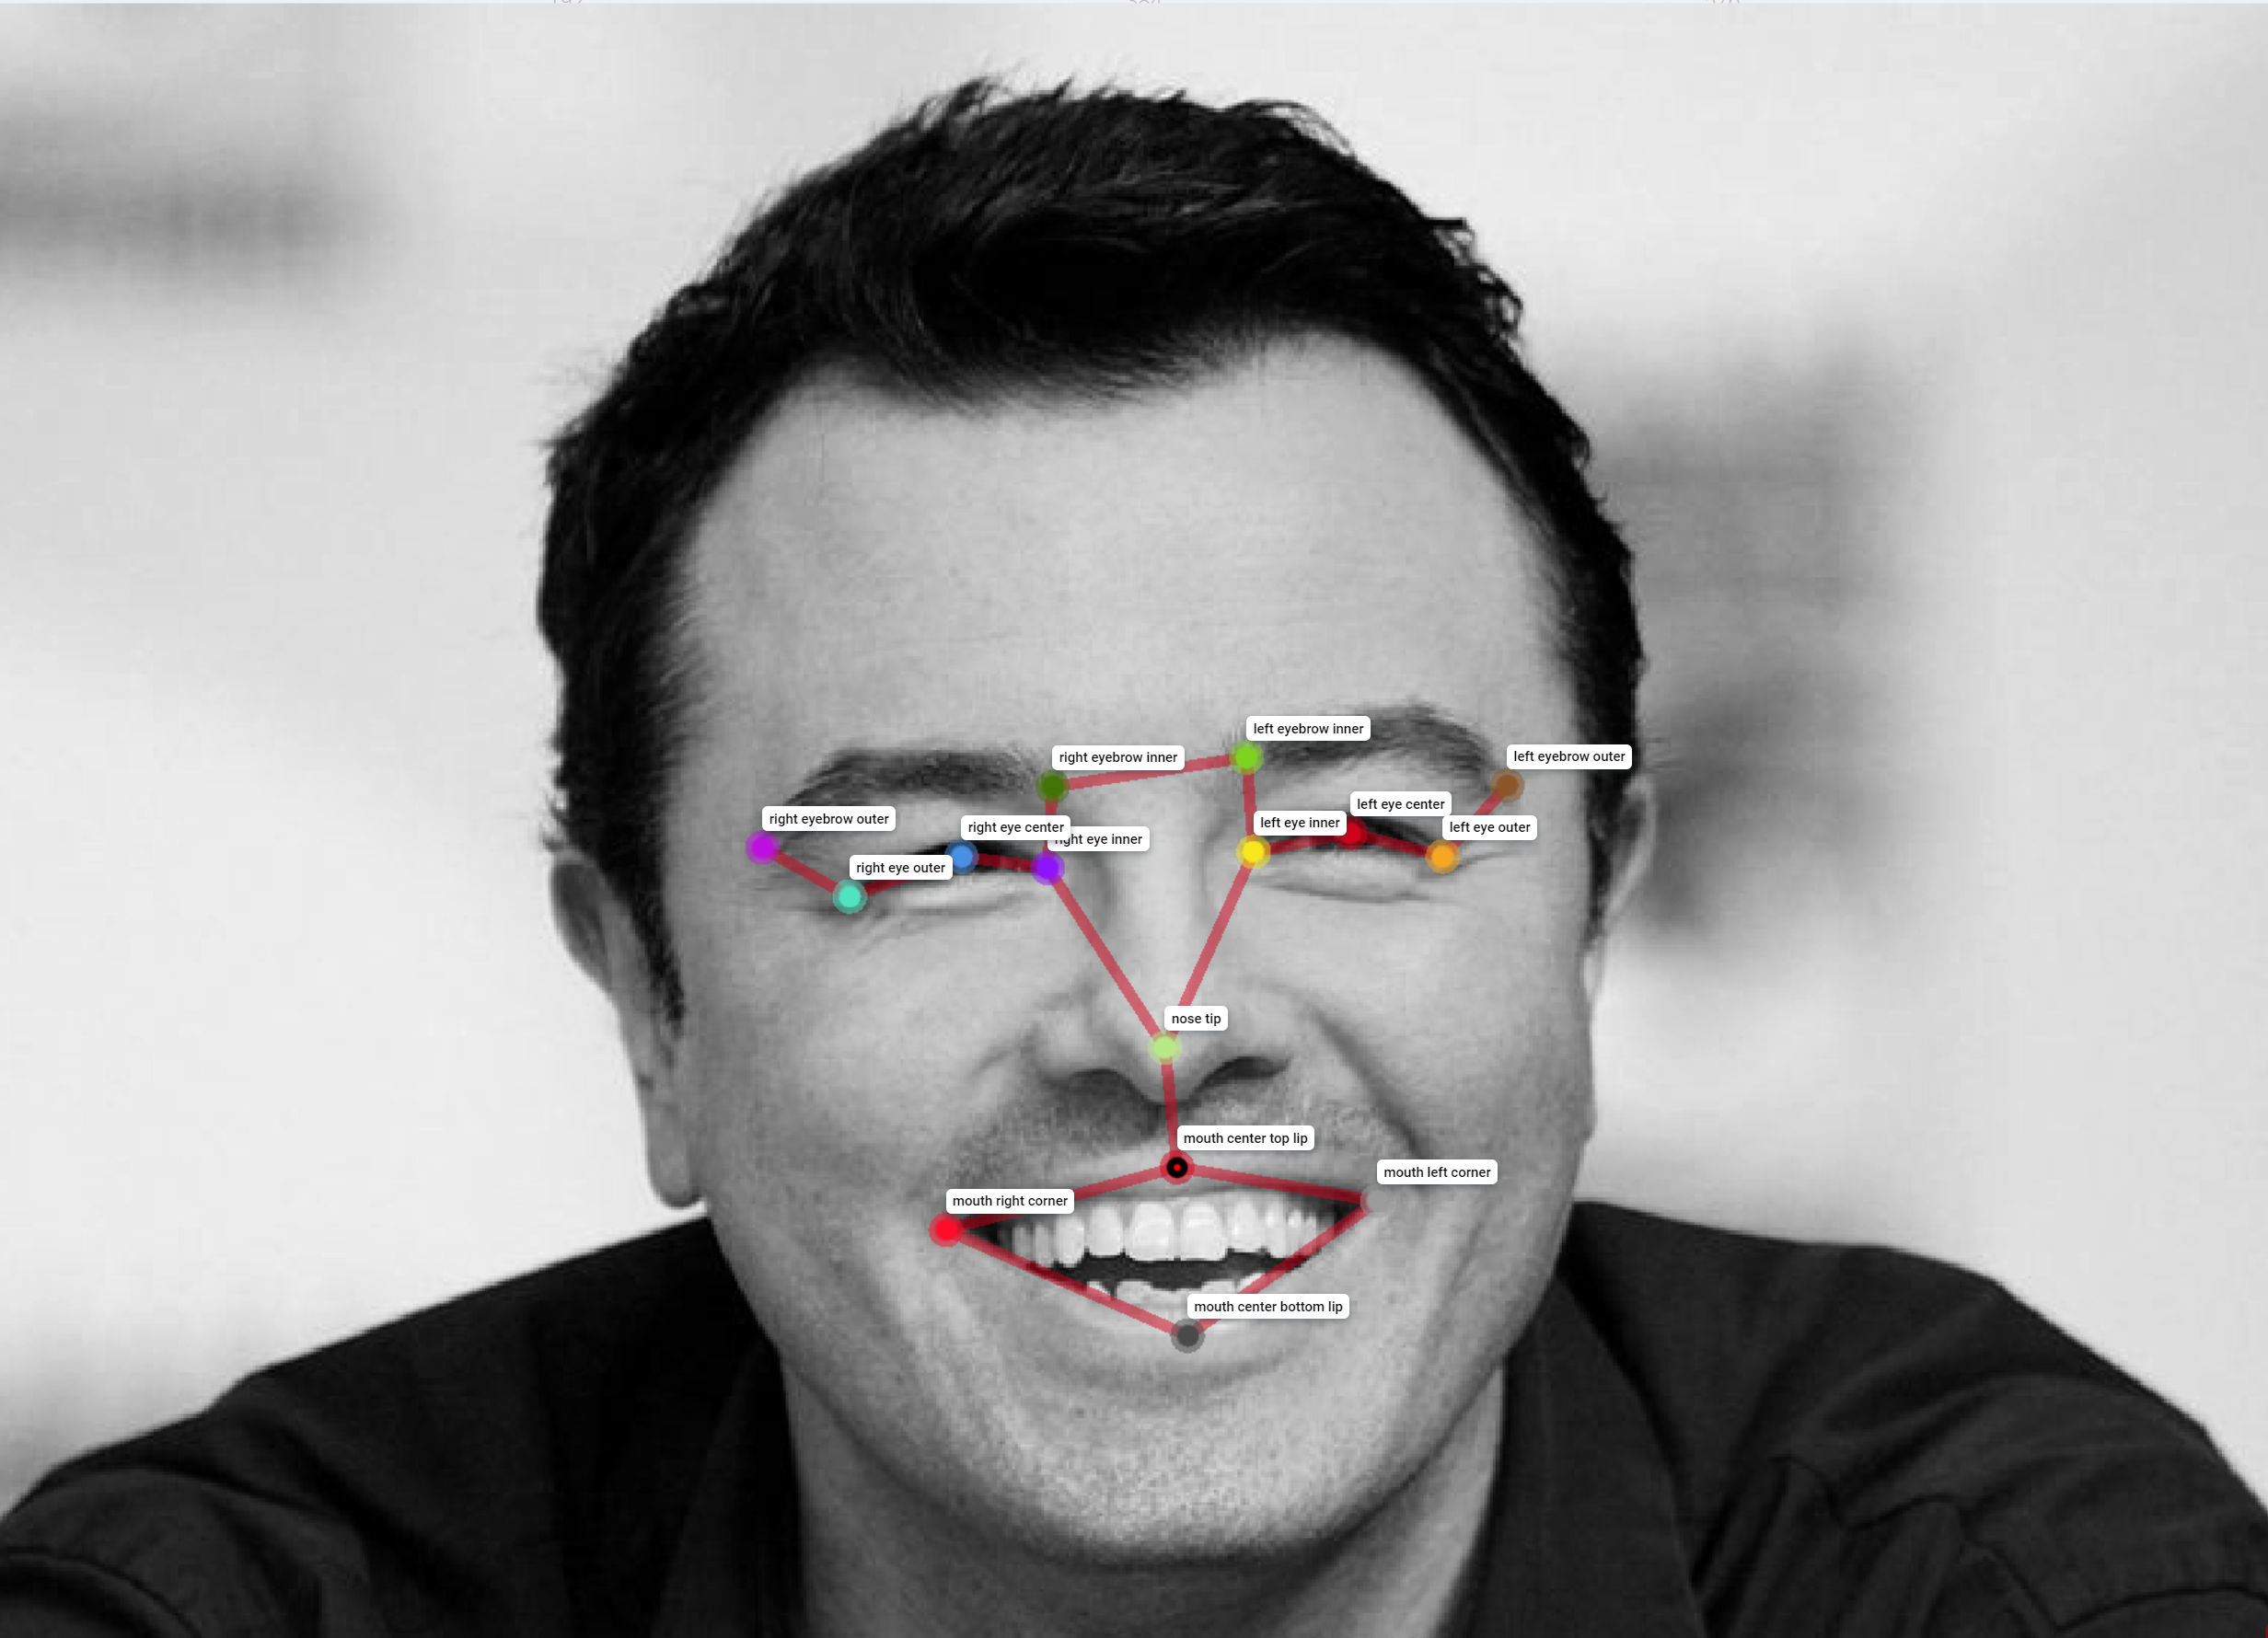
\includegraphics[width=0.95\linewidth]{images/seth.png}
	\caption{Example of 15 facial landmarks labeled on American actor and animator Seth MacFarlane.  This image was not a part of the competition training or test data; rather, it was created to serve as an exemplar inference outcome of our solution.}
	\label{fig:oneexample}
\end{figure}